\paperchapter{August 2017}{27 August 2017}{A}{60}{GSET 2017}
\keytable{\kcell{1}{C} & \kcell{2}{A} & \kcell{3}{D} & \kcell{4}{D} & \kcell{5}{D} & \kcell{6}{C} & \kcell{7}{B} & \kcell{8}{B} & \kcell{9}{C} & \kcell{10}{B} \\
\kcell{11}{D} & \kcell{12}{B} & \kcell{13}{B} & \kcell{14}{C} & \kcell{15}{A} & \kcell{16}{C} & \kcell{17}{D} & \kcell{18}{B} & \kcell{19}{B} & \kcell{20}{D} \\
\kcell{21}{B} & \kcell{22}{B} & \kcell{23}{B} & \kcell{24}{B} & \kcell{25}{A} & \kcell{26}{B} & \kcell{27}{B} & \kcell{28}{A} & \kcell{29}{A} & \kcell{30}{D} \\
\kcell{31}{B} & \kcell{32}{A} & \kcell{33}{C} & \kcell{34}{D} & \kcell{35}{C} & \kcell{36}{B} & \kcell{37}{D} & \kcell{38}{B} & \kcell{39}{B} & \kcell{40}{A} \\
\kcell{41}{B} & \kcell{42}{B} & \kcell{43}{B} & \kcell{44}{D} & \kcell{45}{B} & \kcell{46}{C} & \kcell{47}{D} & \kcell{48}{D} & \kcell{49}{B} & \kcell{50}{B} \\
\kcell{51}{C} & \kcell{52}{D} & \kcell{53}{D} & \kcell{54}{B} & \kcell{55}{C} & \kcell{56}{A} & \kcell{57}{B} & \kcell{58}{B} & \kcell{59}{C} & \kcell{60}{C}}
\begin{question}{1}
{Education would be meaningful when it is \blank{} centric.\par}
\optsfour{Curriculum}{Society}{Student}{Teacher}
\answer{C}{Student}
\begin{explain}
Modern education is \textbf{child-centred (student-centred)}: the curriculum, methods and evaluation are organised around the learner's needs, interests, abilities and pace (Rousseau, Froebel, Dewey, Montessori). Education is meaningful only when it engages the learner actively.
\end{explain}
\end{question}

\begin{question}{2}
{The strength of project method lies in:\par}
\optstwo{Social participation}{Collection of information}{Teacher's instructions}{Individual engagement}
\answer{A}{Social participation}
\begin{explain}
In this paper the official key credits \textbf{social participation}. The project method, developed by W.~H.~Kilpatrick from Dewey's philosophy, has learners work together in groups on real-life, purposeful tasks. Learning thus takes place through cooperation and \emph{social participation}, in a lifelike social setting.
\tip{The same question in GSET Dec 2019 was keyed ``individualised engagement''. Both views are defensible, so always read the options carefully.}
\end{explain}
\end{question}

\begin{question}{3}
{Continuous and comprehensive and scholaristic evaluation means:\par}
\optsone{Scholaristic evaluation of students}{Physical evaluation of students}{Evaluation of students through continuous examination}{Evaluation of overall development of students through continuous evaluation}
\answer{D}{Evaluation of overall development of students through continuous evaluation}
\begin{explain}
\textbf{Continuous and Comprehensive Evaluation (CCE)} evaluates the \textbf{overall (scholastic and co-scholastic) development} of students \textbf{continuously} throughout the year. Continuous means regular formative and summative assessment. Comprehensive means covering cognitive, affective and psychomotor domains (academics, life skills, attitudes, co-curricular activities).
\end{explain}
\end{question}

\begin{question}{4}
{By using audio-visual teaching aids:\par}
\optsone{Students become active in classroom learning}{Teacher becomes active in teaching}{Teaching becomes effective}{All of the above}
\answer{D}{All of the above}
\begin{explain}
Audio-visual aids appeal to several senses at once. They make learners active participants, make the teacher's presentation more dynamic, and so make teaching more effective (``Seeing is believing''; Edgar Dale's Cone of Experience). All three statements are true.
\end{explain}
\end{question}

\begin{question}{5}
{Main objective of diagnostic test, is \blank{}\par}
\optsone{to know the content weakness of student}{to know the scholastic achievement of student}{to do remedial teaching}{(A) and (C) both}
\answer{D}{(A) and (C) both}
\begin{explain}
A \textbf{diagnostic test} pinpoints the specific \textbf{weaknesses or learning difficulties} of a student in the content, and its purpose is to plan \textbf{remedial teaching}. Hence (A) and (C) both.
\why{Measuring overall scholastic achievement is the job of an \emph{achievement} test.}
\end{explain}
\end{question}

\begin{question}{6}
{Who is a better teacher?\par}
\optsone{The one strictly following the disciplinary guidelines}{The one devoting full time to the school}{The one who is interested in overall development of students}{The one who develops quality leadership in his students}
\answer{C}{The one who is interested in overall development of students}
\begin{explain}
The best teacher is concerned with the \textbf{all-round (holistic) development} of students: intellectual, emotional, social, moral and physical. Strict discipline, long hours or leadership training alone are narrower goals.
\end{explain}
\end{question}

\begin{question}{7}
{`Placebo' effect means:\par}
\optstwo{Negative effect}{Positive effect}{Natural effect}{No effect}
\answer{B}{Positive effect}
\begin{explain}
A \textbf{placebo} is an inert treatment (e.g.\ a sugar pill). The \textbf{placebo effect} is the \emph{positive} improvement that occurs simply because the subject believes a treatment is being given. In experiments a placebo group controls for this expectation effect.
\tip{A negative effect produced by negative expectations is called the \emph{nocebo} effect.}
\end{explain}
\end{question}

\begin{question}{8}
{How many variables are there in the factorial research design of 2 $\times$ 3 $\times$ 2?\par}
\optsfour{two}{three}{seven}{twelve}
\answer{B}{three}
\begin{explain}
In a factorial design the notation $2\times3\times2$ gives one number \emph{per independent variable} (factor), each number being the number of levels of that factor. Three numbers mean \textbf{three} variables (with $2\times3\times2=12$ treatment combinations).
\end{explain}
\end{question}

\begin{question}{9}
{In the true experimental research design:\par}
\optsone{No control on external variables}{Less control on external variables}{Control on external variables by randomization}{No use of randomization}
\answer{C}{Control on external variables by randomization}
\begin{explain}
A \textbf{true experimental design} has three features: manipulation of the independent variable, a control group, and \textbf{random assignment} (randomisation), which controls extraneous (external) variables.
\end{explain}
\end{question}

\begin{question}{10}
{What is the full form of APA?\par}
\optstwo{American Philosophical Association}{American Psychological Association}{American Physics Association}{American Pharmacy Association}
\answer{B}{American Psychological Association}
\begin{explain}
\textbf{APA} is the \textbf{American Psychological Association}. Its \emph{Publication Manual} (7th ed., 2019) sets the ``APA style'' of referencing widely used in education and the social sciences.
\end{explain}
\end{question}

\begin{question}{11}
{During the process of data collection from the sample respondents, you obtained some sensitive information, what will be your ethical response in this regard?\par}
\optsone{Sharing the information with family members}{Sharing the information within colleagues}{Sharing the information with general public}{Keeping the information confidential}
\answer{D}{Keeping the information confidential}
\begin{explain}
Research ethics require \textbf{confidentiality}: information from respondents, especially sensitive information, must be kept private and used only for research purposes, with anonymity protected. Sharing it with family, colleagues or the public violates the informed-consent agreement.
\end{explain}
\end{question}

\begin{question}{12}
{In the historical research, external criticism means:\par}
\optstwo{content validity of documents}{validity of originality of documents}{to get information about documents}{to receive documents}
\answer{B}{validity of originality of documents}
\begin{explain}
In historical research, \textbf{external criticism} tests the \textbf{authenticity (genuineness or originality)} of a document or source: is it what it claims to be? (author, date, place, forgery). \textbf{Internal criticism} tests the \emph{credibility, accuracy and meaning of the content}.
\end{explain}
\end{question}

\begin{context}
\textbf{Read the following text and answer the questions 13 to 18.}\par\smallskip
The term `Street Children' is used to refer to children who live on the streets and are deprived of family care and protection. They live in abandoned buildings, containers, automobiles, parks or on street itself. A great deal has been written defining street children. The problem is that there are no precise categories but rather a continuum ranging from children who spend some time in the streets but basically live at home to those who live entirely in the streets and have no adult care. The street children live and work amidst trash, animals and open sewers. They are exposed to many diseases and are unlikely to receive any medical treatment as they cannot afford doctors or medicine. Other major problems of street children are: abuse, child labour, gender discrimination, homelessness and poverty. How can the civil society provide such children their basic constitutional right to health, freedom from violence and abuse is a big challenge.
\end{context}
\begin{question}{13}
{The nature of the above paragraph is:\par}
\optsfour{Analytical}{Descriptive}{Synthesis}{Consequential}
\answer{B}{Descriptive}
\begin{explain}
The paragraph \textbf{describes} who street children are, where they live and the problems they face. It does not analyse causes, synthesise views or trace consequences, so it is \textbf{descriptive}.
\end{explain}
\end{question}

\begin{question}{14}
{The term `Street Children' is a:\par}
\optstwo{Concept}{Definition}{Coined term}{Theoretical framework}
\answer{C}{Coined term}
\begin{explain}
The expression ``street children'' is a \textbf{coined term}: a phrase specially coined (by UNICEF and welfare agencies in the 1980s) to label children who live and work on the streets. The passage itself notes that ``a great deal has been written defining'' them, i.e.\ it is a label rather than a precise definition, concept or theoretical framework.
\end{explain}
\end{question}

\begin{question}{15}
{`Street Children' in this paragraph have been painted as children:\par}
\optstwo{Without home and without parents}{Working as child labourer}{Susceptible to diseases}{Devoid of their basic right}
\answer{A}{Without home and without parents}
\begin{explain}
The opening sentence paints street children as those ``who live on the streets and are deprived of family care and protection'', i.e.\ children \textbf{without home and without parents} (family). The other options (child labour, disease, lack of rights) are consequences mentioned later.
\end{explain}
\end{question}

\begin{question}{16}
{`Street Children' are exposed to many diseases because:\par}
\optstwo{They do not have home}{They have no adult care}{They live near open sewer}{They are discriminated}
\answer{C}{They live near open sewer}
\begin{explain}
According to the official key the main reason is that they \textbf{have no adult care}. With no one to look after them, they live amid trash and sewers and cannot get medical treatment.
\end{explain}
\end{question}

\begin{question}{17}
{Choose the correct answer -- Street children:\par}
\optsone{Live secured life}{They are poor but get care from society}{Get free medical treatment}{Deprived from family care}
\answer{D}{Deprived from family care}
\begin{explain}
Street children are ``\textbf{deprived of family care} and protection'' (first sentence). The other options contradict the passage.
\end{explain}
\end{question}

\begin{question}{18}
{Which one given below is not correct for street children?\par}
\optstwo{They live in abandoned buildings}{They get medical treatment}{They do not get any care}{They are exposed to many diseases}
\answer{B}{They get medical treatment}
\begin{explain}
The passage says they ``are unlikely to receive any medical treatment''. So ``they get medical treatment'' is \textbf{not correct}.
\end{explain}
\end{question}

\begin{question}{19}
{In communication, attributing our own thoughts and feelings to others is called \blank{}\par}
\optsfour{Stereotyping}{Projection}{Halo effect}{Barrier}
\answer{B}{Projection}
\begin{explain}
\textbf{Projection} is the perceptual tendency to attribute one's own thoughts, feelings or motives to others.
\why{Stereotyping judges a person by the group they belong to; the halo effect lets one good trait colour the overall impression.}
\end{explain}
\end{question}

\begin{question}{20}
{Rearrange the steps in order in the process of interpersonal communication:\newline (1) Sender\newline (2) Receiver\newline (3) Message\newline (4) Feedback\newline (5) Channel\newline (6) Encoding\par}
\optsfour{123456}{134265}{132146}{163524}
\answer{D}{163524}
\begin{explain}
The interpersonal communication process in order:
\begin{center}
\begin{tikzpicture}[node distance=2mm,every node/.style={draw=brand,rounded corners,fill=soft,font=\scriptsize,minimum height=6mm}]
\node (a) {Sender (1)}; \node[right=of a] (b) {Encoding (6)}; \node[right=of b] (c) {Message (3)}; \node[right=of c] (d) {Channel (5)}; \node[right=of d] (e) {Receiver (2)}; \node[right=of e] (f) {Feedback (4)};
\foreach \x/\y in {a/b,b/c,c/d,d/e,e/f} \draw[-Stealth,brand] (\x)--(\y);
\end{tikzpicture}
\end{center}
The order is \textbf{1-6-3-5-2-4}, i.e.\ 163524.
\end{explain}
\end{question}

\begin{question}{21}
{The content of communication is called \blank{}\par}
\optsfour{noise}{message}{channel}{distortion}
\answer{B}{message}
\begin{explain}
The \textbf{message} is the content of communication: the information, idea or feeling that the sender wants to convey.
\end{explain}
\end{question}

\begin{question}{22}
{The process by which the receiver interprets the symbols used by the source of message by converting them into concept and ideas is called \blank{}\par}
\optsfour{Encoding}{Decoding}{Listening}{Speaking}
\answer{B}{Decoding}
\begin{explain}
\textbf{Decoding}: the receiver interprets the symbols and converts them back into concepts and ideas.
\end{explain}
\end{question}

\begin{question}{23}
{The main purpose of communication is to impart \blank{}\par}
\optsfour{Training}{Information}{Discipline}{Skill}
\answer{B}{Information}
\begin{explain}
The primary purpose of communication is to impart (share) \textbf{information}. Training, discipline and skills are specific outcomes that depend on communicating information.
\end{explain}
\end{question}

\begin{question}{24}
{Which of the following is the most effective way of communication?\par}
\optstwo{Verbal communication}{Written communication}{Non-verbal communication}{Silence}
\answer{B}{Written communication}
\begin{explain}
The official key gives \textbf{written communication}: it is precise, permanent, verifiable, can reach many people and can be referred to repeatedly, which makes it the most reliable and effective form, especially in formal settings.
\end{explain}
\end{question}

\begin{question}{25}
{Find out the next term in the following series:\newline 0, 3, 8, 15, 24, \ldots{}\par}
\optsfour{35}{32}{39}{37}
\answer{A}{35}
\begin{explain}
Each term is $n^2-1$: $1-1=0$, $4-1=3$, $9-1=8$, $16-1=15$, $25-1=24$, so next $36-1=\mathbf{35}$. (Differences: 3, 5, 7, 9, 11.)
\end{explain}
\end{question}

\begin{question}{26}
{Find the missing number in the following:\par}
\qfigure{\begin{tabular}{|c|c|c|}\hline 0 & 2 & 4\\\hline 1 & 3 & 5\\\hline 7 & 9 & 11\\\hline 0 & 24 & ?\\\hline\end{tabular}}
\optsfour{20}{64}{59}{29}
\answer{B}{64}
\begin{explain}
Work column by column: bottom $=$ top $\times$ (sum of the two middle numbers).
\[0\times(1+7)=0,\qquad 2\times(3+9)=24,\qquad 4\times(5+11)=\mathbf{64}\]
\end{explain}
\end{question}

\begin{question}{27}
{If HEALTH is written as GSKZDG, then how will NORTH be written in that code?\par}
\optsfour{OPSUI}{GSQNM}{FRPML}{IUSPO}
\answer{B}{GSQNM}
\begin{explain}
HEALTH $\rightarrow$ GSKZDG: \emph{reverse} the word (HTLAEH) and then move each letter \emph{one step back}: H$\rightarrow$G, T$\rightarrow$S, L$\rightarrow$K, A$\rightarrow$Z, E$\rightarrow$D, H$\rightarrow$G.
NORTH reversed is HTRON; one step back gives \textbf{GSQNM}.
\end{explain}
\end{question}

\begin{question}{28}
{If L stands for (+), M stands for (--), N stands for ($\times$) and P stands for ($\div$), then 14N 10L 42P 2M 8 = ?\par}
\optsfour{153}{216}{248}{251}
\answer{A}{153}
\begin{explain}
Substituting: $14\times10+42\div2-8=140+21-8=\mathbf{153}$.
\end{explain}
\end{question}

\begin{question}{29}
{A person's age is 3 times more than the age of his friend. The total of their ages is 64 years. Find the ages of the person and his friend:\par}
\optsfour{48, 16}{16, 64}{64, 16}{22, 42}
\answer{A}{48, 16}
\begin{explain}
The key reads ``3 times more than'' as ``3 times''. Friend $=x$, person $=3x$, $4x=64\Rightarrow x=16$. The ages are \textbf{48 and 16}.
\end{explain}
\end{question}

\begin{question}{30}
{If (A + B) > (C + D) and (B + C) > (A + D), then it is definite that:\par}
\optsfour{D > B}{C > D}{A > D}{B > D}
\answer{D}{B > D}
\begin{explain}
Add the two inequalities:
\[(A+B)+(B+C)>(C+D)+(A+D)\ \Rightarrow\ A+2B+C>A+C+2D\ \Rightarrow\ B>D\]
So \textbf{B $>$ D} is definite.
\end{explain}
\end{question}

\begin{question}{31}
{In the following question there is a certain relationship between two given words of one side of :: and one word on the other side of it, choose the correct alternative:\newline Aryabhatta : Mathematician :: Varahmihira : ?\par}
\optsfour{Physician}{Astronomer}{Scientist}{Architect}
\answer{B}{Astronomer}
\begin{explain}
Aryabhata was a mathematician (and astronomer); \textbf{Varahamihira} (6th century, \emph{Pancha-Siddhantika}, \emph{Brihat-Samhita}) is best known as an \textbf{astronomer} and astrologer.
\end{explain}
\end{question}

\begin{question}{32}
{Study the diagram below and identify the region representing youth who are employed but not educated:\par}
\qfigure{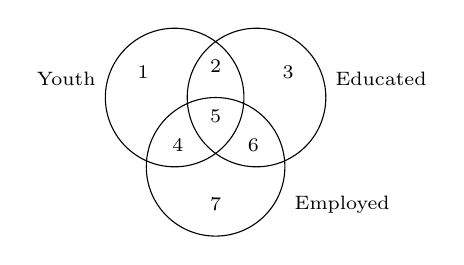
\begin{tikzpicture}[scale=0.8,font=\scriptsize]
\draw (0,0.5) circle(1.1); \draw (1.3,0.5) circle(1.1); \draw (0.65,-0.6) circle(1.1);
\node at (-0.5,0.9){1}; \node at (0.65,1.0){2}; \node at (1.8,0.9){3}; \node at (0.05,-0.25){4}; \node at (0.65,0.2){5}; \node at (1.25,-0.25){6}; \node at (0.65,-1.2){7};
\node[left] at (-1.1,0.8){Youth}; \node[right] at (2.4,0.8){Educated}; \node[right] at (1.75,-1.2){Employed};
\end{tikzpicture}}
\optsfour{4 only}{5, 6}{1, 4, 7}{4, 7}
\answer{A}{4 only}
\begin{explain}
The required region is \emph{inside} Youth, \emph{inside} Employed and \emph{outside} Educated. Only region \textbf{4} satisfies all three conditions.
\why{5 is also educated, 6 is not youth, and 7 is employed only (not youth).}
\end{explain}
\end{question}

\begin{question}{33}
{The question below consists of two statements numbered I and II. You have to decide whether the data provided in the statements are sufficient to answer the question.\\
\textbf{How is Tanya related to the man in the photograph?}\\
(I) Man in the photograph is the only son of Tanya's grandfather.\\
(II) The man in photograph has no brothers or sisters and his father is Tanya's grandfather.\par}
\optsone{Statement I alone is sufficient, II is not}{Statement II alone is sufficient, I is not}{Either statement I or II alone is sufficient}{Both statements together are not sufficient}
\answer{C}{Either statement I or II alone is sufficient}
\begin{explain}
The official key holds that each statement alone establishes that the man is the only son of Tanya's grandfather, and therefore \textbf{Tanya's father}. (Strictly, Tanya could also be a daughter's child; the setters assume the paternal line.) Both statements give the same information, so \textbf{either I or II} alone suffices.
\end{explain}
\end{question}

\begin{question}{34}
{How many triangles are there in the following figure?\par}
\qfigure{\begin{tikzpicture}[scale=0.9,font=\scriptsize]
\coordinate (A) at (0,2.5); \coordinate (B) at (-2,0); \coordinate (C) at (2,0); \coordinate (D) at (0,0);
\coordinate (O) at (0,0.95); \coordinate (E) at ($(A)!0.449!(C)$);
\draw[thick] (A)--(B)--(C)--cycle; \draw[thick] (A)--(D); \draw[thick] (B)--(E); \draw[thick] (C)--(O);
\foreach \p/\pos in {A/above,B/left,C/right,D/below,O/left,E/right} \node[\pos] at (\p) {\p};
\end{tikzpicture}}
\optsfour{6}{10}{11}{12}
\answer{D}{12}
\begin{explain}
Label the points as in the figure. The lines are AB, AC (through E), BC (through D), AD (through O), BE (through O) and CO. The triangles are:
\begin{center}\small
ABD, ABO, ABC, ABE, ADC, AOC, AOE, BOD, BOC, BEC, ODC, OEC
\end{center}
Total $=$ \textbf{12}.
\end{explain}
\end{question}

\begin{question}{35}
{In the following question, four words have been given, out of which three are alike in some manner and the fourth one is different. Choose the odd one.\par}
\optsfour{Veena}{Sitar}{Drum}{Guitar}
\answer{C}{Drum}
\begin{explain}
Veena, sitar and guitar are \textbf{string} instruments; the \textbf{drum} is a percussion instrument, so it is the odd one out.
\end{explain}
\end{question}

\begin{question}{36}
{In the question below, there are two statements labelled as Assertion (A) and Reason (R).\\
\textbf{Assertion (A):} Indian President is the head of country.\\
\textbf{Reason (R):} Indian Parliament consists of the President, Lok Sabha and Rajya Sabha.\par}
\optsone{If both (A) and (R) are true and (R) is the correct explanation of (A)}{Both (A) and (R) are true but (R) is not the correct explanation of (A)}{(A) is true (R) is false}{(A) is false (R) is true}
\answer{B}{Both (A) and (R) are true but (R) is not the correct explanation of (A)}
\begin{explain}
Both statements are true. The President is the constitutional Head of State (Art.~52--53), and Parliament consists of the President and the two Houses (Art.~79). But being part of Parliament is not \emph{why} the President is head of the country, so R does not explain A.
\end{explain}
\end{question}

\begin{question}{37}
{The bar graph given below shows the percentage distribution of total expenditure of a company under various expense heads during 2015. Study the graph and answer the questions that follows:\par}
\qfigure{\begin{tikzpicture}
\begin{axis}[ybar,width=10cm,height=4.4cm,bar width=13pt,ymin=0,ymax=25,
  symbolic x coords={Infrastructure,Transport,Advertisements,Taxes,R\&D,Salary,Interest on loans},xtick=data,
  x tick label style={rotate=30,anchor=east,font=\scriptsize},yticklabel style={font=\scriptsize},
  nodes near coords,every node near coord/.append style={font=\tiny},ylabel={\scriptsize Percent spent},
  axis x line*=bottom,axis y line*=left]
\addplot[fill=white,draw=ink] coordinates {(Infrastructure,20) (Transport,12.5) (Advertisements,15) (Taxes,10) (R\&D,5) (Salary,20) (Interest on loans,17.5)};
\end{axis}
\end{tikzpicture}}
The expenditures on the interests on loans is by what percentage more than the expenditures on transport?
\optsfour{10\%}{20\%}{30\%}{40\%}
\answer{D}{40\%}
\begin{explain}
Interest on loans $=17.5\%$; transport $=12.5\%$.
\[\frac{17.5-12.5}{12.5}\times100=\frac{5}{12.5}\times100=\mathbf{40\%}\]
\end{explain}
\end{question}

\begin{question}{38}
{The following pie-chart shows the sources of funds to be collected by the National Highways Authority of India (NHAI) for its phase-II projects. Study the pie-chart and answer the question that follow:\par}
\qfigure{\begin{tikzpicture}\pie[radius=1.4,text=pin,hide number,font=\scriptsize,color={brand!10,brand!30,brand!15,brand!40,brand!5}]{19.94/External Assistance 11{,}486,9.12/SPVS 5{,}252,8.52/Toll 4{,}910,10.42/Annuity 6{,}000,52/Market borrowing 29{,}952}\end{tikzpicture}}
Total funds to be arranged for projects (phase II) $=$ Rs.~57,600 crores. The approximate ratio of funds to be arranged through toll and that through market borrowing is:
\optsfour{2 : 9}{1 : 6}{3 : 11}{2 : 5}
\answer{B}{1 : 6}
\begin{explain}
\[\frac{\text{Toll}}{\text{Market borrowing}}=\frac{4910}{29952}\approx\frac{1}{6.1}\approx\mathbf{1:6}\]
\end{explain}
\end{question}

\begin{question}{39}
{A researcher wants to study the association between gender and using a mobile phone. Data collected for this study will be \blank{}\par}
\optstwo{Quantitative data}{Qualitative data}{Continuous data}{Classified data}
\answer{B}{Qualitative data}
\begin{explain}
Gender (male/female) and mobile-phone use (user/non-user) are \textbf{categorical attributes}, i.e.\ qualities rather than measured quantities. The data are therefore \textbf{qualitative (nominal)}, typically analysed with a chi-square test of association.
\end{explain}
\end{question}

\begin{question}{40}
{A Government agency responsible for collection of various types of data in India is CSO. What is its full form?\par}
\optstwo{Central Statistical Office}{Central Statistical Organisation}{Central State Organisation}{Central Staff Organisation}
\answer{A}{Central Statistical Office}
\begin{explain}
\textbf{CSO} was the \textbf{Central Statistics Office} under the Ministry of Statistics and Programme Implementation (MoSPI), and the key's ``Central Statistical Office'' is this body. It compiled national accounts, GDP, IIP, CPI and so on. In 2019 it merged with the NSSO to form the \emph{National Statistical Office (NSO)}.
\end{explain}
\end{question}

\begin{question}{41}
{In order to show the strengths of PG and Ph.D. students in TEN different institutions of a state, most suitable diagram will be:\par}
\optstwo{Pie chart}{Two pie charts}{Multiple bar diagram}{Two Multiple bar diagrams}
\answer{B}{Two pie charts}
\begin{explain}
The official key gives \textbf{two pie charts}. Each chart shows how one category, PG students in one and PhD students in the other, is distributed among the ten institutions, i.e.\ each institution's share. (A multiple-bar diagram would be the choice for comparing absolute numbers side by side.)
\end{explain}
\end{question}

\begin{question}{42}
{The following table gives the percentage distribution of five states: P, Q, R, S and T on the basis of poverty line and also on the basis of gender. Study the table and answer the question:\par}
\qfigure{\small
\begin{tabular}{c c cc}\toprule
& & \multicolumn{2}{c}{\textbf{Males : Females}}\\\cmidrule(l){3-4}
\textbf{State} & \textbf{\% below poverty line} & \textbf{Below PL} & \textbf{Above PL}\\\midrule
P & 35 & 5 : 6 & 6 : 7\\ Q & 25 & 3 : 5 & 4 : 5\\ R & 24 & 1 : 2 & 2 : 3\\ S & 19 & 3 : 2 & 4 : 3\\ T & 15 & 5 : 3 & 3 : 2\\\bottomrule
\end{tabular}}
What will be the number of females above poverty line in the state S if it is known that population of state S is 7 million?
\optsfour{3 million}{2.43 million}{1.33 million}{5.7 million}
\answer{B}{2.43 million}
\begin{explain}
State S: above poverty line $=100-19=81\%$ of 7 million $=5.67$ million.
Females : males above PL $=3:(4+3)$, so females $=\tfrac37\times5.67=\textbf{2.43 million}$.
\end{explain}
\end{question}

\begin{question}{43}
{Created by Kevin Systrome and Mike Kriger, this app was acquired by facebook in April 2012, what it is?\par}
\optsfour{Twitter}{Instagram}{Whatsapp}{Linkedin}
\answer{B}{Instagram}
\begin{explain}
\textbf{Instagram} was created by Kevin Systrom and Mike Krieger (launched October 2010) and acquired by Facebook in April 2012 for about US\$1 billion.
\end{explain}
\end{question}

\begin{question}{44}
{`NPTEL' a project funded by MHRD, Govt. of India represents \blank{}\par}
\optsone{National Productivity Technique of Educational Leadership}{National Programme of Telephone Emergency Locator}{North Province Teacher Education Library}{National Programme on Technology Enhanced Learning}
\answer{D}{National Programme on Technology Enhanced Learning}
\begin{explain}
\textbf{NPTEL} is the \textbf{National Programme on Technology Enhanced Learning}, a joint initiative of the IITs and IISc funded by MHRD (since 2003). It offers online courses in engineering and science and is a SWAYAM national coordinator.
\end{explain}
\end{question}

\begin{question}{45}
{URL provides a standard hierarchical way of identifying and locating internet resources on World Wide Web (www). What does URL stand for?\par}
\optstwo{Uniform Recurrence Locator}{Uniform Resource Locator}{Uniform Remote Locator}{Uniform Revised Locator}
\answer{B}{Uniform Resource Locator}
\begin{explain}
\textbf{URL} is \textbf{Uniform Resource Locator}, the web address of a resource, e.g.\ \texttt{https://www.example.com/index.html} (protocol, domain, path).
\end{explain}
\end{question}

\begin{question}{46}
{It is a unique numeric identifier used to specify a particular host computer on a particular network, what it is?\par}
\optsfour{LP address}{UP address}{IP address}{IL address}
\answer{C}{IP address}
\begin{explain}
An \textbf{IP (Internet Protocol) address} is the unique numerical label assigned to each device on a network. IPv4 addresses are 32-bit (e.g.\ 192.168.1.1); IPv6 addresses are 128-bit.
\end{explain}
\end{question}

\begin{question}{47}
{This symbol was introduced by Ray Tomlinson in 1971. What it is?\par}
\optsfour{!}{\%}{\$}{@}
\answer{D}{@}
\begin{explain}
\textbf{Ray Tomlinson} sent the first network e-mail on ARPANET in 1971 and chose the \textbf{``@''} symbol to separate the user name from the host name.
\end{explain}
\end{question}

\begin{question}{48}
{HTML stands for:\par}
\optstwo{High text markup language}{Hypertext marketing language}{Hypertext makeup language}{Hypertext markup language}
\answer{D}{Hypertext markup language}
\begin{explain}
\textbf{HTML} is \textbf{HyperText Markup Language}, the standard language for creating web pages, devised by Tim Berners-Lee (1991).
\end{explain}
\end{question}

\begin{question}{49}
{Which plant is used in biodiesel?\par}
\optsfour{Palm tree}{Jatropha}{Coconut tree}{Eucalyptus}
\answer{B}{Jatropha}
\begin{explain}
\textbf{Jatropha curcas} is the main non-edible oilseed plant promoted for biodiesel in India (National Mission on Biodiesel, 2003). It grows on wasteland and does not compete with food crops.
\end{explain}
\end{question}

\begin{question}{50}
{Global environmental problem is mainly due to:\par}
\optstwo{Climate change}{Increasing population}{Rising temperature}{Melting of Iceberg}
\answer{B}{Increasing population}
\begin{explain}
The official key gives \textbf{increasing population}. A growing population drives higher consumption of resources, pollution, deforestation and emissions, and so underlies most global environmental problems. Climate change, rising temperature and melting icebergs are its \emph{consequences}.
\end{explain}
\end{question}

\begin{question}{51}
{Pesticide fertilizer causes which pollution?\par}
\optstwo{Air pollution}{Water pollution}{Soil pollution}{Oil pollution}
\answer{C}{Soil pollution}
\begin{explain}
Pesticides and chemical fertilisers applied to fields accumulate in the soil, alter soil chemistry, kill soil organisms and leave toxic residues. Their direct impact is \textbf{soil pollution}, though run-off can also pollute water.
\end{explain}
\end{question}

\begin{question}{52}
{Lead tetraethyl is added to gasoline to make:\par}
\optstwo{gasoline thin}{to increase its speed}{to decrease fumes}{because of antiknock property}
\answer{D}{because of antiknock property}
\begin{explain}
\textbf{Tetraethyl lead (TEL)} was added to petrol as an \textbf{anti-knock agent}. It raises the octane rating and prevents premature ignition (knocking) in engines. It was banned because it emits toxic lead; India phased out leaded petrol by 2000.
\end{explain}
\end{question}

\begin{question}{53}
{Which will not come under natural hazards?\par}
\optstwo{Flood}{Volcanic eruption}{Earthquake}{Plane crash}
\answer{D}{Plane crash}
\begin{explain}
Floods, volcanic eruptions and earthquakes are \textbf{natural} hazards. A \textbf{plane crash} is a \emph{man-made (technological)} disaster.
\end{explain}
\end{question}

\begin{question}{54}
{Which is not true for disturbing natural environment?\par}
\optstwo{Deforestation}{Afforestation}{Development of coastal zones}{Urban development}
\answer{B}{Afforestation}
\begin{explain}
Deforestation, development of coastal zones and urbanisation disturb the natural environment. \textbf{Afforestation} (planting trees) \emph{restores} the environment, so it is the one that does not disturb it.
\end{explain}
\end{question}

\begin{question}{55}
{Which one of the following is a Women's University?\par}
\optstwo{Gujarat University}{Gujarat Vidyapeeth}{Banasthali Vidyapeeth}{Sardar Patel University}
\answer{C}{Banasthali Vidyapeeth}
\begin{explain}
\textbf{Banasthali Vidyapith} (Rajasthan, founded 1935) is one of the largest residential \textbf{women's universities} in the world.
\why{Gujarat University, Gujarat Vidyapith and Sardar Patel University are co-educational.}
\end{explain}
\end{question}

\begin{question}{56}
{Which of the following was declared as an institution of national importance in India?\par}
\optsone{National Institute of Design, Ahmedabad}{Institution of Rural Management, Anand}{Pandit Deendayal Petroleum University, Gandhinagar}{Entrepreneurship Development Institute of India, Gandhinagar}
\answer{A}{National Institute of Design, Ahmedabad}
\begin{explain}
The \textbf{National Institute of Design (NID), Ahmedabad} was declared an \textbf{Institution of National Importance} by the NID Act, 2014.
\end{explain}
\end{question}

\begin{question}{57}
{NCTE is responsible for the quality of \blank{} in India.\par}
\optstwo{Technical Education}{Teacher Education}{Computer Education}{Commerce and Trade Education}
\answer{B}{Teacher Education}
\begin{explain}
The \textbf{National Council for Teacher Education (NCTE)} became a statutory body under the NCTE Act, 1993. It regulates norms, standards and quality in \textbf{teacher education} (B.Ed., D.El.Ed., M.Ed.).
\end{explain}
\end{question}

\begin{question}{58}
{What is the full form of NEET, an examination for admission into medical courses in India?\par}
\optstwo{National Employment Emergency Test}{National Eligibility cum Entrance Test}{National Entrance and Eligibility Test}{National Energy Efficient Test}
\answer{B}{National Eligibility cum Entrance Test}
\begin{explain}
\textbf{NEET} is the \textbf{National Eligibility cum Entrance Test} for admission to MBBS, BDS and allied courses, conducted by the NTA.
\end{explain}
\end{question}

\begin{question}{59}
{What is the full form of NAAC?\par}
\optsone{National Authority for Assessing Colleges}{National Accreditation Authority Council}{National Assessment and Accreditation Council}{National Agency for Accreditation of Colleges}
\answer{C}{National Assessment and Accreditation Council}
\begin{explain}
\textbf{NAAC} is the \textbf{National Assessment and Accreditation Council}, established in 1994 by UGC, Bengaluru.
\end{explain}
\end{question}

\begin{question}{60}
{Which Educational institute was declared the best in the over all India rankings 2017?\par}
\optsone{The Maharaja Sayajirao University of Baroda, Vadodara}{Banaras Hindu University, Varanasi}{Indian Institute of Science, Bangalore}{Indian Institute of Management, Ahmedabad}
\answer{C}{Indian Institute of Science, Bangalore}
\begin{explain}
In \textbf{NIRF 2017} (India Rankings), the \textbf{Indian Institute of Science, Bengaluru} was ranked first in the \emph{Overall} category.
\end{explain}
\end{question}
